\chapter{Methodology}\label{formulation}

This chapter first explains the theory and assumptions behind small-signal analysis of the inverters and then elaborates on the mathematical linearization and derivation of the small-signal matrix form of each function in an inverter. Finally, it summarizes the full small-signal model by presenting a matrix form block diagram representation.

\section{Background Theory and Procedure}\label{theory}

In the future 100\% inverter-based power system, system inertia will be low; therefore, the inter-area oscillations may remain undamped for a long time. This work in the first phase is to build comprehensive small-signal model of the inverter-based resources, which would be used to analyze system stability and solve the problems of the inter-area oscillation damping. The general approach for inter-area oscillation can be summarized in three steps.
\begin{itemize}
    \item Derivation of equivalent small-signal output inductance model for a single inverter
    \item Order reduction of the resultant equivalent small-signal output inductance to enable computational and visual inter-area oscillation analysis.
    \item 	Integration of order reduced equivalent small-signal output inductance model to derive small-signal modes and performing tuning to improve the overall system damping.
\end{itemize}

In this thesis, the focus is on the modeling part of the mentioned procedure. However, precautions are taken to make it readily available for eigenvalue analysis and model reduction. Therefore, the equivalent impedance/admittance matrix approach has been used instead of the commonly used state-space model. This approach makes the inverter level order reduction significantly easier. In addition, it allows the different elements of the circuit to be added to multiple inverter sets in a modular manner.


Certain assumptions are made in order to make the system able to rely on small-signal model in specific phenomena. For example, all protection systems, such as current limiting and fault ride-through controls, are neglected during a small-signal oscillation. In addition, because the study is on the transmission and generation side, the anti-islanding protections which specific for distribution inverters are not considered. Dynamics of the input energy source is neglected and considered slow. Therefore, the DC side is considered as an equivalent capacitor and a constant input current. It is also assumed that if a perturbation happens in the magnitude of \gls{PWM} input, the output perturbation is not affected by the high-frequency terms, and therefore switching frequencies can be neglected. It is assumed that the $V_{ref}$ and $\theta_{ref}$ are determined by the optimal power flow studies at the system level, which is slower than system dynamics.

 It needs to be mentioned that the frequency perturbation is only considered as a dependent variable to output voltages or currents rather than an independent variable, and no independent changes in the frequency are assumed.


The main theory behind equivalent impedance/admittance modeling is that the poles of the equivalent impedance/admittance transfer functions are identical to the eigenvalues of the inverter.

Because the inverters are considered to be three-phase and balanced, they can be transformed into $dq$ frame for control purposes. For example, voltage, current, and modulation index that are inherently complex signals will be shown as a $2\times 1$ matrix containing both $d$ and $q$ axis components. System signals such as angle and DC voltage are converted into the matrix format to obtain a generalized formulation for each block. Because of the couplings between $d$ and $q$ frames on the controller side, the corresponding impedance/admittance or the block equivalent gain must be a $2 \times 2$ matrix. 
For example, the conversion for impedance formulation will become:

\begin{equation}
\Delta V=Z_{out} \Delta I
\end{equation}
where: 
\begin{equation}
Z_{out}=\left[\begin{matrix}Z_{out}^{dd}&Z_{out}^{dq}\\Z_{out}^{qd}&Z_{out}^{qq}\\\end{matrix}\right]
\end{equation}
and
\begin{equation}
\Delta V=\left[\begin{matrix}V_d\\V_q\end{matrix}\right] \end{equation}and \begin{equation}\Delta I=\left[\begin{matrix}I_d\\I_q\end{matrix}\right]
 \end{equation}
where:

\begin{equation}
\begin{split}
\Delta V_d=Z^{dd}_{out} \Delta I_d+Z^{dq}_{out}\Delta I_q\\  \Delta V_q=Z^{qd}_{out}\Delta I_d+Z^{qq}_{out}\Delta I_q
\end{split}
\end{equation}




\section{Small-Signal Approximation of Inverters}\label{smallsignal}

In this section, small-signal formulation of each part in inverter model is presented based on the theory mentioned in \ref{theory}

The prime-suffixed variables denotes the measured variables in the local $dq$ frame. The difference between local and global $dq$ frames which are explicitly shown in \ref{dq}. 

\subsection{Output Filter}

\subsubsection{The L filert}
For L filter the $dq$ matrix form equation is:

\begin{equation}\label{lfilter}
\Delta V_o - U= \begin{bmatrix} sL & -L\omega \\ L\omega & sL\end{bmatrix}\Delta I
\end{equation}
where $L$ is the inductance of the inductor, $s$ is the Laplace variable and the $\omega$ is the system frequency. The variables are $\Delta V_o$, output voltage, $\Delta U$, inverter's voltage, and $\Delta I$, the inverter's current perturbations. \ref{lfilter} can be written in matrix form as:
\begin{equation}
\Delta V_o - U_c= \mathbf{Z_L} \Delta I_o
\end{equation}
where  $\mathbf{Z_L}$ is the inductor's impedance in the matrix form.
\subsubsection{The LCL filert}
For LCL filter the $dq$ matrix form equation is:
\begin{equation}
\Delta V_o - V_c= \begin{bmatrix} sL_2 & -L_2\omega \\ L_2\omega & sL_2\end{bmatrix} \Delta I_o
\end{equation}
\begin{equation}
 \Delta I_o-\Delta I = \begin{bmatrix} sC & -C\omega \\ C\omega & sC\end{bmatrix}\Delta V_c 
\end{equation}
\begin{equation}
 \Delta U-\Delta V_c = \begin{bmatrix} sL_1 & -L_1\omega \\ L_1\omega & sL_1\end{bmatrix}\Delta I 
\end{equation}

which can be written in matrix form as:

\begin{equation}
\Delta V_o - V_c=\mathbf{\mathbf{Z_L_2} } \Delta I_o
\end{equation}
\begin{equation}
 \Delta I_o-\Delta I = \mathbf{Z_c } \Delta V_c 
\end{equation}
\begin{equation}
 \Delta U-\Delta V_c = \mathbf{Z_L_1 } \Delta I 
\end{equation}

\subsection{\gls{PWM}}

In reality, the PWM block is the inverter itself that takes the input from the controls and converts it into a duty cycle for the switching device. This switching of DC voltage with varying duty cycles makes a controlled output AC voltage after low-pass filtering. The assumption here is that the high frequency is neglected in the small-signal, and the average model for switching devices is inherently used. The main equation for the PWM block is: 

\begin{equation}\label{PWM}
 U=INV*V_{DC}D
\end{equation}
where $D$ is the modulation index and $U$ is the output voltage. Both $D$ and $U$ are considered in $dq$ frame as $D=\begin{bmatrix}D_d \\ D_q \end{bmatrix}$ and $U=\begin{bmatrix}U_d \\ U_q \end{bmatrix}$. The \ref{PWM} is nonlinear and must be linearized for small-signal analysis. The $*$ operator denotes simple matrix multiplication.


\begin{equation}\label{PWM2}
 U+\Delta U=INV*(V_{DC}+\Delta V_{DC})(D+ \Delta D)
\end{equation}
where $INV=\begin{bmatrix}\frac{1-0.5T_{del}s}{1+0.5T_{del}s} & 0 \\ 0 & \frac{1-0.5T_{del}s}{1+0.5T_{del}s}\end{bmatrix}$ is the switching delay transfer function in the matrix form and
\begin{equation}\label{PWM2}
 U+\Delta U=INV*((V_{DC})(D)+(V_{DC})(\Delta D)+(\Delta V_{DC})(D)+(\Delta V_{DC})(\Delta D))
\end{equation}

By neglecting steady-state and double incremental terms we obtain:

\begin{equation}\label{PWM2}
\Delta U=INV*((V_{DC})(\Delta D)+(\Delta V_{DC})(D))
\end{equation}

Finally,
\begin{equation}\label{PWM3}
\Delta U=Delv*\Delta D+Deld*\Delta V_{DC}
\end{equation}

in which $Delv=INV*V_{DC}$ and $Deld=INV*D$

\subsection{Current Loop}
Inner current loop is a linear block that controls the input of PWM with its reference current and can be seen in \ref{cr}.

\begin{equation}\label{cr}
\Delta D'=\begin{bmatrix}PI_c & 0 \\ 0 & PI_c \end{bmatrix}(\Delta I_{ref}-\Delta I')+\begin{bmatrix}0 & -L_1\omega \\ L_1\omega & 0 \end{bmatrix}\Delta I'+\begin{bmatrix}fv & 0 \\ 0 & fv \end{bmatrix}V'_c
\end{equation}

and the final matrix form equation can be derived as:

\begin{equation}\label{cr2}
\Delta D'=PIC(\Delta I_{ref}-\Delta I')+L1w*\Delta I'+FV*V'_c
\end{equation}

\subsection{Voltage/Power Loop}
\textit{Power Loop in GFL:} Power loop is used in GFL to provide a constant active and reactive power:
\begin{equation}\label{pr}
\Delta I_{ref}=\begin{bmatrix}PI_p & 0 \\ 0 & PI_q \end{bmatrix}(\Delta S_{ref}-\Delta S)
\end{equation}
which  can be rewritten in the matrix form as:

\begin{equation}\label{pr2}
\Delta I_{ref}=PIS*(\Delta S_{ref}-\Delta S)
\end{equation}
\textit{Voltage Loop in GFM:} Voltage loop is used in GFM in order to control the voltage:
\begin{equation}\label{vr}
\Delta I_{ref}=\begin{bmatrix}PI_v & 0 \\ 0 & PI_v \end{bmatrix}(\Delta V_{ref} -\Delta V'_c)+\begin{bmatrix}0 & -C\omega \\ C\omega & 0 \end{bmatrix}\Delta V'_c+\begin{bmatrix}fc & 0 \\ 0 & fc \end{bmatrix}\Delta I'
\end{equation}
By assuming that the $V_{ref}=constant$, \ref{vr} can be reduce to:

\begin{equation}\label{vr2}
\Delta I_{ref}=-\begin{bmatrix}PI_v & 0 \\ 0 & PI_v \end{bmatrix}\Delta V'_c+\begin{bmatrix}0 & -C\omega \\ C\omega & 0 \end{bmatrix}\Delta V'_c+\begin{bmatrix}fc & 0 \\ 0 & fc \end{bmatrix}\Delta I'
\end{equation}
Therefore, The matrix form of \ref{vr} is:
\begin{equation}\label{vr3}
\Delta I_{ref}=-PIV*\Delta V'_c+Cw*\Delta V'_c+F_I_I*\Delta I'
\end{equation}

\subsection{Power Measurement}
Power measurements in terms of $I'_d$, $I'_q$, $V'_d$, and $V'_q$ are:

\begin{equation}
 P=\frac{\omega_c}{s+\omega_c}(V'_dI'_d+V'_qI'_q)
\end{equation}

\begin{equation}
 Q=\frac{\omega_c}{s+\omega_c}(V'_qI'_d-V'_dI'_q)
\end{equation}
where $pfilter=\frac{\omega_c}{s+\omega_c}$ is a low-pass filter for measurement. This is a nonlinear block, and it needs to be linearized in order to be used in small-signal analysis. The linearization has been done as follows:

\begin{equation}\label{p1}
 P+\Delta P=pfilter((V'_d+\Delta V'_d)(I'_d+\Delta I'_d)+(V'_q+\Delta V'_q)(I'_q+\Delta I'_q))
\end{equation}

\begin{equation}\label{p2}
 Q+\Delta Q=pfilter((V'_q+\Delta V'_q)(I'_d+\Delta I'_d)-(V'_d+\Delta V'_d)(I'_q+\Delta I'_q))
\end{equation}

\cref{p1,p2} can be elaborated as:
\begin{equation}
\begin{split}
 P+\Delta P=pfilter((V'_d)(I'_d)+(V'_q)(I'_q)+(\Delta V'_d)(I'_d)+(\Delta V'_q)(I'_q)+(V'_d)(\Delta I'_d)\\+(V'_q)(\Delta I'_q)+(\Delta V'_d)(\Delta I'_d)+(\Delta V'_q)(\Delta I'_q))
 \end{split}
\end{equation}

\begin{equation}
\begin{split}
  Q+\Delta Q=pfilter((V'_q)(I'_d)-(V'_d)(I'_q)+(\Delta V'_q)(I'_d)-(\Delta V'_d)(I'_q)+(V'_q)(\Delta I'_d)\\-(V'_d)(\Delta I'_q)+(\Delta V'_q)(\Delta I'_d)-(\Delta V'_d)(\Delta I'_q))
   \end{split}
\end{equation}

If the large signal and double incremental terms are dropped, the equation will become:

\begin{equation}
 \Delta P' =pfilter((I'_d)(\Delta V'_d)+(I'_q)(\Delta V'_q)+(V'_d)(\Delta I'_d)+(V'_q)(\Delta I'_q))
\end{equation}

\begin{equation}
 \Delta Q' =pfilter((I'_d)(\Delta V'_q)-(I'_q)(\Delta V'_d)+(V'_q)(\Delta I'_d)-(V'_d)(\Delta I'_q))
\end{equation}
which can be rewritten as:

\begin{equation}\label{power}
 \Delta P' =pfilter(\begin{bmatrix}I'_d & I'_q\end{bmatrix}\begin{bmatrix}\Delta V'_d\\\Delta V'_q\end{bmatrix}+\begin{bmatrix}V'_d & V'_q\end{bmatrix}\begin{bmatrix}\Delta I'_d\\\Delta I'_q\end{bmatrix})
\end{equation}

\begin{equation}
 \Delta Q'  =pfilter(\begin{bmatrix}-I'_q & I'_d\end{bmatrix}\begin{bmatrix}\Delta V'_d\\\Delta V'_q\end{bmatrix}+\begin{bmatrix}V'_q & -V'_d\end{bmatrix}\begin{bmatrix}\Delta I'_d\\\Delta I'_q\end{bmatrix})
\end{equation}

and finally,

\begin{equation}\label{power2}
 \Delta S =\begin{bmatrix}pfilter & 0\\0 &  pfilter\end{bmatrix}(\begin{bmatrix}I'_d & I'_q\\-I'_q & I'_d\end{bmatrix}\begin{bmatrix}\Delta V'_d\\\Delta V'_q\end{bmatrix}+\begin{bmatrix}V'_d & V'_q\\V'_q & -V'_d\end{bmatrix}\begin{bmatrix}\Delta I'_d\\\Delta I'_q\end{bmatrix})
\end{equation}

We assume $Io=\begin{bmatrix}I'_d & I'_q\\-I'_q & I'_d\end{bmatrix}$,  $Vo=\begin{bmatrix}V'_d & V'_q\\V'_q & -V'_d\end{bmatrix}$ and $Pfilter=\begin{bmatrix}pfilter & 0\\0 &  pfilter\end{bmatrix}$ to derive the matrix form:
\begin{equation}\label{p3}
\Delta S =Pfilter(Io \Delta V'+Vo \Delta I')
\end{equation}
\subsection{DC-side Dynamics}

Based on the law of conservation of energy, i.e., $W_{DC}=W_{AC}$, we have:

\begin{equation}
 \Delta W_{DC}=\Delta W_{AC}
\end{equation}

\begin{equation}\label{DC}
 \Delta W_{DC}=\Delta ({\frac{1}{2}(C_{DC})V^2_{DC}})
\end{equation}
A linearization must be performed to implement the \ref{DC} which can be derived as:
\begin{equation}
 \Delta W_{DC}= {C_{DC}V_{DC}\Delta V_{DC}}
\end{equation}
In time domain:
\begin{equation}
 \Delta W_{DC}= \Delta W_{AC}= \int{\Delta P_{AC}}dt
\end{equation}
and in frequency domain:

\begin{equation}
 \Delta W_{DC} = \frac{\Delta P_{AC}}{s}
\end{equation}

\begin{equation}
 {C_{DC}V_{DC}\Delta V_{DC}} = \frac{\Delta P_{AC}}{s}
\end{equation}

By assuming that $\Delta P'_{AC}=\Delta P'$ and also $\Delta V_{dc}=\begin{bmatrix}\Delta V_{DC} \\ 0 \end{bmatrix}$ we obtain:

\begin{equation}
 {C_{DC}V_{DC}\Delta V_{DC}} = \frac{\Delta P'}{s}
\end{equation}

\begin{equation}
 \Delta V_{DC} = \frac{\Delta P'}{C_{DC}V_{DC}s}
\end{equation}

\begin{equation}
 \Delta V_{dc} = \begin{bmatrix}\Delta V_{DC} \\ 0\end{bmatrix}
\end{equation}

\begin{equation}
 \Delta V_{dc} =\begin{bmatrix}\frac{1}{C_{DC}V_{DC}s} & 0 \\ 0 & 0\end{bmatrix} {\Delta S}
\end{equation}

\begin{equation}\label{DCfinal}
 \Delta V_{dc} =DC {\Delta S}
\end{equation}
By plugging \ref{power2} into \ref{DCfinal}:
\begin{equation}
 \Delta V_{dc} =Kdc \Delta V'+Zdc \Delta I'
\end{equation}
where $Zdc=DC*Io$ and $Kdc=DC*Vo$

\begin{figure}[ht]
    \centering
	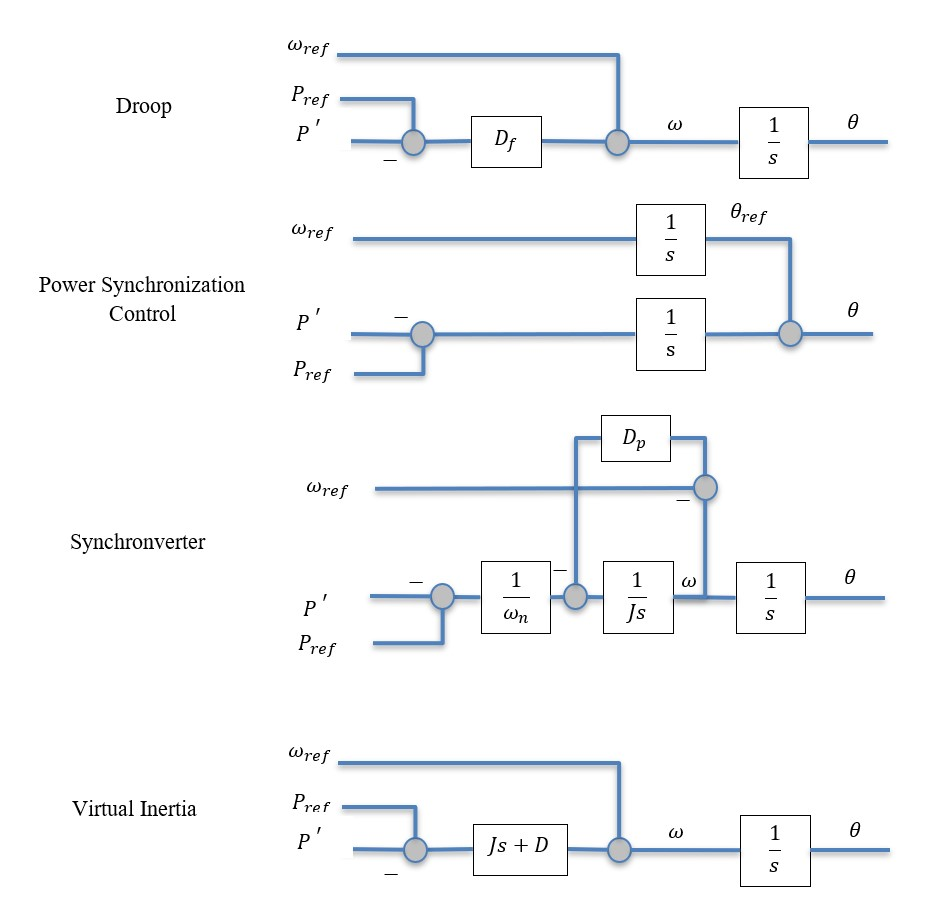
\includegraphics[width=0.85\textwidth]{figures/strategies.jpg}
	\caption[GFM strategies for angle generation]{GFM strategies for angle generation}
	\label{strategies}
\end{figure}

\subsection{Angle Reference Generation}\label{Inverters}
Angle reference is a necessary input for $abc/dq$ and $dq/abc$ blocks in an inverter which can be generated via different methods in different GFM and GFL inverters. \ref{strategies} shows control blocks of different GFM strategies for angle generation. This subsection derives the small-signal model of these angle generation blocks.

\subsubsection{GFL-Conventional}
In the conventional basic GFL in which $\theta=Constant$, we have:
\begin{equation}\label{thetatot}
 \Delta \theta=0 
\end{equation}
In order to have a consistant modeling, a new complex variable named $\Delta \theta$ is introduced instead of $\Delta \theta$ 
\begin{equation}
 \Delta T=\begin{bmatrix}0 \\ \Delta \theta \end{bmatrix}
\end{equation}
Therefore, for the conventional GFL, we have:
\begin{equation}
\Delta T=\begin{bmatrix}0  \\ 0 \end{bmatrix}
\end{equation}



\subsubsection{GFL-PLL}
In most of the GFLs, angle reference that is used in $dq/abc$ or $abc/dq$ blocks are generated via \gls{PLL}. PLL equation is:
\begin{equation}\label{deltatheta}
    \Delta \theta=(PI_{pll}/s)\Delta V'_q
\end{equation}
 \cref{PLL1,PLL2,PLL3} convert PLL equation into $\Delta T$ form: 
\begin{equation}\label{PLL1}
    \Delta \theta=\begin{bmatrix}(0 & PI_{pll}/s)\end{bmatrix}\Delta V'_q
\end{equation}
\begin{equation}\label{PLL2}
 \Delta T=\begin{bmatrix}0 & 0 \\ 0 & PI_{pll}s\end{bmatrix}\Delta V'   
\end{equation}
\begin{equation}\label{PLL3}
\Delta T=PLL*\Delta V'
\end{equation}




\subsubsection{GFM - Droop Control}


Droop control resembles the speed droop property of
the governor and trades off deviations of the power
injection and frequency deviations from their nominal value \cite{comparison}:



\begin{equation}
\Delta \theta=\frac{D_f}{s}\Delta P
\end{equation}
\begin{equation}
 \Delta T=\begin{bmatrix}0 & 0 \\ \frac{D_f}{s} &  0\end{bmatrix}\Delta S   
\end{equation}
\begin{equation}
\Delta T=DroopGFM *\Delta S
\end{equation}

\subsubsection{GFM - Syn}
\gls{Syn} is a well-known strategy that satisfies the
need for a synchronization unit for pre-synchronization
purposes, as well as and during normal operation \cite{comparison2}.
\begin{equation}
\Delta \theta=\frac{1}{sJ\omega_n(s+\frac{D_p}{J(1+D_pPI_ps)})}\Delta P
\end{equation}
\begin{equation}
 \Delta T=\begin{bmatrix}0 & 0 \\ \frac{1}{sJ\omega_n(s+\frac{D_p}{J(1+D_pPI_ps)})} &  0\end{bmatrix}\Delta S   
\end{equation}
\begin{equation}
\Delta T=SYN *\Delta S
\end{equation}
\subsubsection{GFM - Virtual Inertia}
The \gls{VIL} control is a control strategy in which to avoid switching from self-synchronization mode to
PLL-mode during grid faults, the use of a PLL is also foreseen during normal operation. Indeed, the output frequency
is continuously provided by the PLL, whereas the angle $\theta$ is calculated according to a particular equation \cite{comparison2} that can be converted to the small-signal as:
\begin{equation}
\Delta \theta=\frac{1}{Js^2+Ds}\Delta P
\end{equation}
\begin{equation}
 \Delta T=\begin{bmatrix}0 & 0 \\ \frac{1}{JS^2+Ds} &  0\end{bmatrix}\Delta S   
\end{equation}
\begin{equation}
\Delta T=\gls{VIL}*\Delta S
\end{equation}

\subsubsection{GFM - PSC}
The \gls{PSC} is another control strategy where second-order transfer function is implemented in the inner frequency loop, acting on the deviation between power
setpoint and measured power \cite{comparison2}.
\begin{equation}
\Delta \theta=\frac{K_i}{s}\Delta P
\end{equation}

\begin{equation}
 \Delta T=\begin{bmatrix}0 & 0 \\ \frac{K_i}{s} &  0\end{bmatrix}\Delta S   
\end{equation}

\begin{equation}
\Delta T=\gls{PSC}\Delta S
\end{equation}


\subsection{$abc/dq$ and inverse transform}\label{dq}
To properly control the inverter, a $abc/dq$ transfer is necessary. A global $dq$ frame must be considered when considering oscillation between multiple inverters. Both voltage and current signals are converted into a local $dq$ frame to be able to control and then create a global $dq$ frame output. During transients, these two frames may not be exactly the same because of the angle dynamics. In addition, because of the large grid assumption, there is also a steady-state angle difference between both voltage and current global and local $dq$ frames. In this study we will index the local dq frame signals with a prime symbol to distinguish it from the global frame signals.
\subsubsection{$abc/dq$ transform:} $abc/dq$ transform in global $dq$ frame is:
\begin{equation}\label{}
A'=e^{j\theta}A
\end{equation}
both $\theta$ and $A$ values can be perturbed. Therefore, small-signal perturbation of transferred value must consist of both terms. The linear approximation is derived as follows:
\begin{equation}\label{}
A'+\Delta A'=e^{j(\theta+\Delta \theta)}(A+\Delta A)
\end{equation}
\begin{equation}\label{}
A'+\Delta A'\approx e^{j\theta}(1+\Delta \theta)(A+\Delta A)
\end{equation}
\begin{equation}\label{xx}
A'+\Delta A'\approx e^{j\theta}(A+\Delta \theta A+\Delta A + \Delta \theta \Delta A)
\end{equation}
By dropping the steady-state and double incremental terms \ref{xx} will become:





\begin{equation}\label{}
\Delta A'\approx e^{j\theta}( A \Delta \theta+ \Delta A)
\end{equation}

\begin{equation}\label{}
e^{j\theta} A' \Delta \theta= (cos\theta+j sin\theta) (A_d+j A_q) \Delta \theta
\end{equation}

\begin{equation}\label{}
e^{j\theta} A' \Delta \theta= ((cos\theta A_d - A_q sin\theta) + j (sin\theta A_d+ cos\theta A_d)) \Delta \theta
\end{equation}

\begin{equation}\label{}
e^{j\theta} A' \Delta \theta=\begin{bmatrix} (cos\theta A_d - A_q sin\theta) \\ (sin\theta A_d+ cos\theta A_d) \end{bmatrix}\Delta \theta
\end{equation}

\begin{equation}\label{}
\begin{bmatrix}\Delta A'_d\\\Delta A'_q\end{bmatrix}\approx \begin{bmatrix} (cos\theta A_d - A_q sin\theta) \\ (sin\theta A_d+ cos\theta A_d) \end{bmatrix}\Delta \theta +  \begin{bmatrix}cos\theta & -sin\theta\\sin\theta & cos\theta\end{bmatrix}  \begin{bmatrix}\Delta A_d\\\Delta A_q\end{bmatrix}
\end{equation}

considering \ref{thetatot}, and converting it into matrix, we obtain:

\begin{equation}\label{}
\begin{bmatrix}\Delta A'_d\\\Delta A'_q\end{bmatrix}\approx \begin{bmatrix} 0 & (cos\theta A_d - A_q sin\theta) \\ 0 & (sin\theta A_d+ cos\theta A_d) \end{bmatrix}\begin{bmatrix}0 \\\Delta \theta \end{bmatrix}+  \begin{bmatrix}cos\theta & -sin\theta\\sin\theta & cos\theta\end{bmatrix}  \begin{bmatrix}\Delta A_d\\\Delta A_q\end{bmatrix}
\end{equation}

\begin{equation}\label{}
\Delta A'\approx T_A \Delta T+  T_{main} \Delta A
\end{equation}

Finally, the $A$ variable can be replaced with the output voltage and currrent variables:

\begin{equation}\label{}
\Delta V_o'= T_V \Delta T+  T_{main} \Delta V
\end{equation}

\begin{equation}\label{}
\Delta I_o'= T_I \Delta T+  T_{main} \Delta I
\end{equation}

\begin{equation}\label{}
\Delta V_c'= T_V_c \Delta T+  T_{main} \Delta V_c
\end{equation}

\subsubsection{$dq/abc$ transform:} Similarly in the inverse conversion we have

\begin{equation}\label{}
A=e^{-j\theta}A'
\end{equation}
\begin{equation}\label{}
A+\Delta A=e^{-j(\theta+\Delta \theta)}(A'+\Delta A')
\end{equation}
\begin{equation}\label{}
A+\Delta A\approx e^{-j\theta}(1-\Delta \theta)(A'+\Delta A')
\end{equation}
\begin{equation}\label{yy}
A+\Delta A\approx e^{-j\theta}(A'-\Delta \theta A'+\Delta A' - \Delta \theta \Delta A')
\end{equation}
By dropping the steady-state and double incremental terms \ref{yy} will become:





\begin{equation}\label{}
\Delta A\approx e^{-j\theta}( \Delta A' - A' \Delta \theta)
\end{equation}

\begin{equation}\label{}
e^{-j\theta} A \Delta \theta= (cos\theta-j sin\theta) (A'_d+j A'_q) \Delta \theta
\end{equation}

\begin{equation}\label{}
e^{-j\theta} A \Delta \theta= ((cos\theta A'_d + A'_q sin\theta) + j (-sin\theta A'_d+ cos\theta A'_d)) \Delta \theta
\end{equation}

\begin{equation}\label{}
e^{j\theta} A \Delta \theta=\begin{bmatrix} (cos\theta A'_d + A'_q sin\theta) \\ (-sin\theta A'_d+ cos\theta A'_d) \end{bmatrix}\Delta \theta
\end{equation}

\begin{equation}\label{zz}
\begin{bmatrix}\Delta A_d\\\Delta A_q\end{bmatrix}\approx \begin{bmatrix} (cos\theta A'_d + A'_q sin\theta) \\ (-sin\theta A'_d+ cos\theta A'_d) \end{bmatrix}\Delta \theta +  \begin{bmatrix}cos\theta & sin\theta\\-sin\theta & cos\theta\end{bmatrix}  \begin{bmatrix}\Delta A'_d\\\Delta A'_q\end{bmatrix}
\end{equation}

considering \ref{thetatot}, matrix conversion of \ref{zz} will become:

\begin{equation}\label{}
\begin{bmatrix}\Delta A_d\\\Delta A_q\end{bmatrix}\approx \begin{bmatrix} 0 & (cos\theta A'_d + A'_q sin\theta) \\ 0 & (-sin\theta A'_d+ cos\theta A'_d) \end{bmatrix}\begin{bmatrix}0 \\\Delta \theta \end{bmatrix}+  \begin{bmatrix}cos\theta & sin\theta\\-sin\theta & cos\theta\end{bmatrix}  \begin{bmatrix}\Delta A'_d\\\Delta A'_q\end{bmatrix}
\end{equation}

\begin{equation}\label{}
\Delta A\approx T_A' \Delta T+  1/T_{main} \Delta A
\end{equation}

Finally, the actual modulation index formula can be obtained in the matrix form as: 

\begin{equation}\label{}
\Delta D = T_D' \Delta T+  1/T_{main} \Delta D'
\end{equation}

\subsection{GFL - Droop}

Some GFLs also participate in the voltage and frequency support to the system via GFL droop block which adjusts active and reactive power references based on frequency, and voltage magnitude, respectively. The corresponding equation will be: \cref{GFLdroop-1,GFLdroop0}:

\begin{equation}\label{GFLdroop-1}
\Delta P_{ref}={\Delta \theta}/m_p
\end{equation}
\begin{equation}\label{GFLdroop0}
\Delta Q_{ref}={\Delta V_m}/n_p
\end{equation}
\begin{equation}\label{GFLdroop1}
\Delta S_{ref}=\begin{bmatrix} P_{ref} \\ Q_{ref}  \end{bmatrix}
\end{equation}

$V_m$ is the output voltage magnitude, which can be written as $V_m=\sqrt{(V^2_d+V^2_q)}$ and can be linearized as:
\begin{equation}\label{GFLdroop3}
\Delta V_m=(V_d/V_m)\Delta V'_d + (V_q/V_m)\Delta V'_q
\end{equation}
The prime indices are added to $\Delta V_m$ to indicate that it is generated from voltage measurements. $\Delta \theta$ is also calculated in \ref{deltatheta}. Resultant  $\Delta P_{ref}$ $\Delta Q_{ref}$ $\Delta S_{ref}$ can be derived as:
\begin{equation}\label{sref1}
\Delta P_{ref}=\begin{bmatrix}0 & PI_{pll}/{sm_p}\end{bmatrix}\Delta V'
\end{equation}
\begin{equation}\label{sref2}
\Delta Q_{ref}=\begin{bmatrix} V_d/{V_mn_p} & V_q/{V_mn_p}\end{bmatrix}\Delta V'
\end{equation}

\begin{equation}\label{sref3}
\Delta S_{ref}=\begin{bmatrix} 0 & PI_{pll}/{sm_p} \\ V_d/{V_mn_p} & V_q/{V_mn_p}\end{bmatrix}\Delta V'
\end{equation}

\begin{equation}\label{sref4}
\Delta S_{ref}=DroopGFL\Delta V'
\end{equation}
\section{Section Summary}

\ref{fig:model} summarizes block diagram representation of both \gls{GFM} and \gls{GFL} inverter complex models. In \ref{fig:model} each signal is a $2 \times 1$ matrix (for example $ \begin{bmatrix}\Delta V_d \\ \Delta V_q \end{bmatrix} $ $ \begin{bmatrix}\Delta I_d \\ \Delta I_q \end{bmatrix} $ $ \begin{bmatrix}\Delta P \\ \Delta Q \end{bmatrix} and \begin{bmatrix}\Delta \theta \\ 0\end{bmatrix}$) and each transfer block is a $2\times2$ matrix of transfer functions, $ \begin{bmatrix}Xdd & Xdq \\Xqd & Xqq\end{bmatrix} $ or a linear function of two $2\times2$ matrices when there are two inputs ($ A\begin{bmatrix}Xdd & Xdq \\Xqd & Xqq\end{bmatrix}+B\begin{bmatrix}Ydd & Ydq \\Yqd & Yqq\end{bmatrix} $). In \ref{fig:model}, the red parts are only for \gls{GFL} converters, and blue characters are only for GFM converters. The linearized block diagrams are shown in \ref{fig:lin}.

As shown in the \ref{fig:model}, the small-signal model of the GFL converter is built considering the $abc/dq$ effect. Under voltage disturbance, this block generates an error between the converter and global $dq$ frames. The effect of $\Delta T$ on the measured small-signal currents and voltages in both GFL and GFM topology is shown. The noticeable point in \ref{fig:model} is how the generation of $\Delta T$ is different in GFL and GFM. The figure shows that the GFM $\Delta T$ is generated using both $\Delta I$ and $\Delta V$ signals, whereas the GFL $\Delta T$ is only made from $\Delta V$. Therefore, complexity doubles in the GFM, and more poles will be added to the final small-signal impedance.

  The difference between GFM and GFL is the existence of $\Delta I$ alongside $\Delta V$ in reference angle generation. The way that this extra term affects the number of poles will be further discussed in \ref{numberofpoles}.

\begin{figure}[ht]
    \centering
	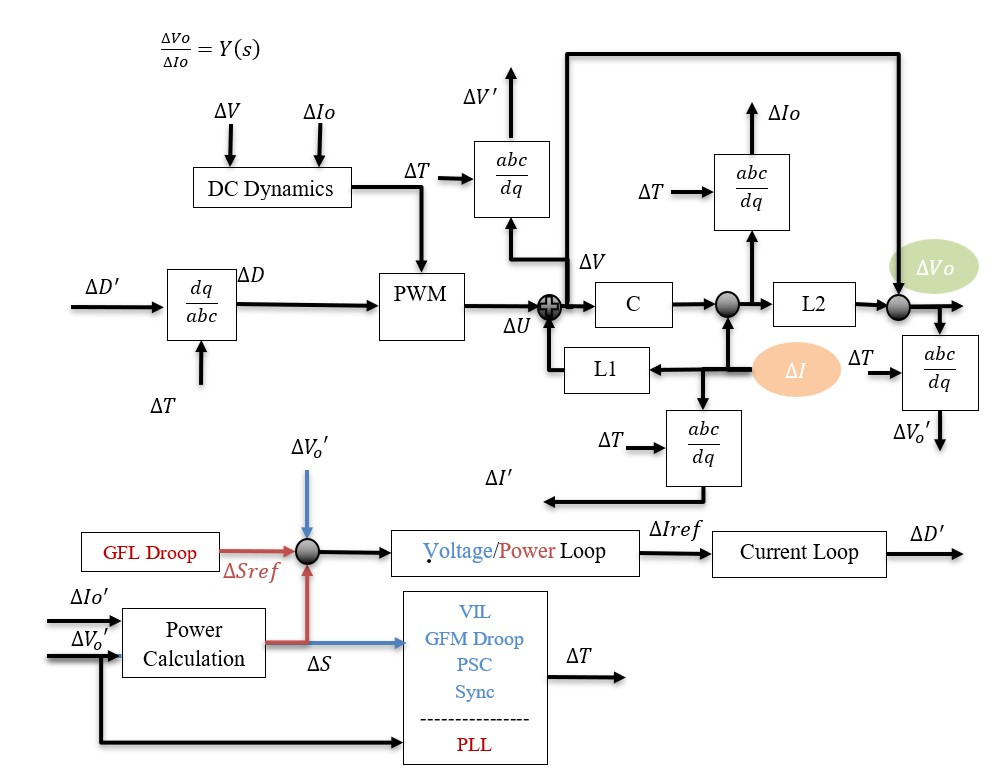
\includegraphics[width=0.85\textwidth]{figures/Inverter Model.jpg}
	\caption[Exact Inverter Models]{Exact Inverter small-signal model in matrix form. Black lines and text are for both GFM and GFL, blue lines and text are only for GFM, and red lines and text are only for GFL.}
	\label{fig:model}
\end{figure}

\begin{figure}[ht]
    \centering
	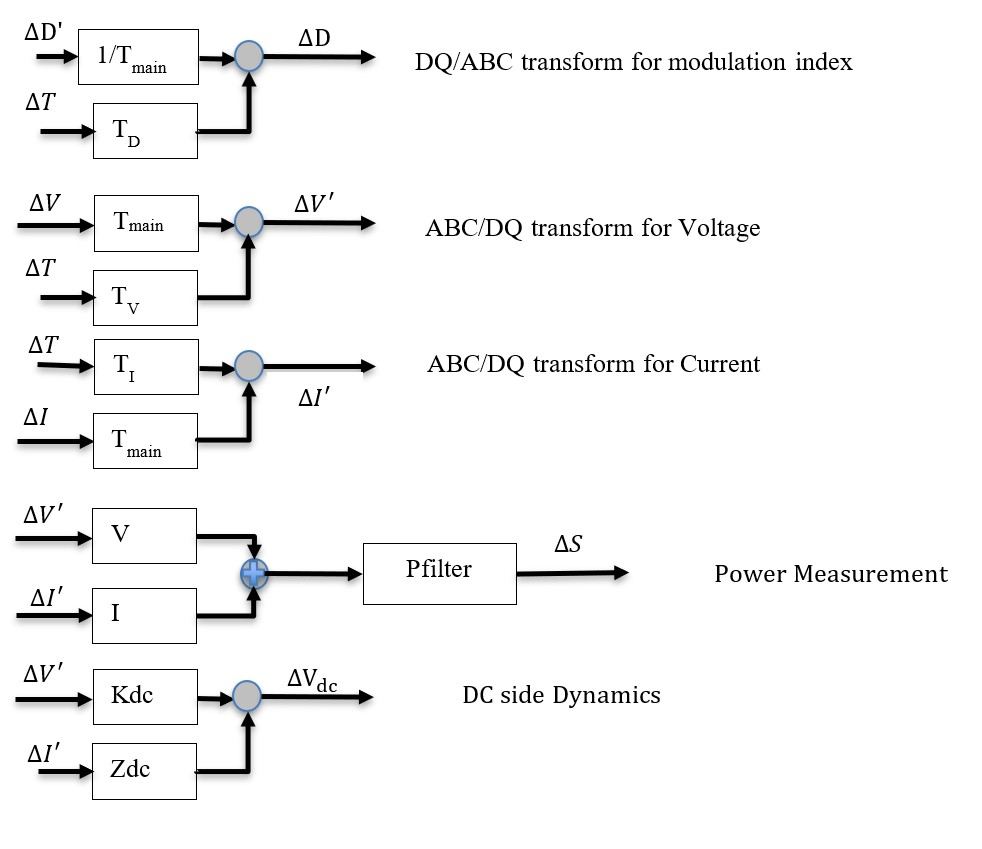
\includegraphics[width=0.85\textwidth]{figures/Inverter lin.jpg}
	\caption[Liniearized Block Diagrams]{Linearized block diagrams of the inverters.}
	\label{fig:lin}
\end{figure}
